\chapter{Thực hành từng bước trên Fiji/ImageJ}\label{chap:fiji}
\section{Dữ liệu, mục tiêu và nhật ký thực hành}
Fiji/ImageJ và MorphoLibJ 1.6.5 được dùng như nền tảng tham chiếu \cite{ref1,ref2}. Phần này đi từ ảnh gốc đến ảnh nhãn bằng menu Fiji, không cần mở MorphoLab hoặc dùng Python tạo trước các đầu vào Watershed. Sau khi làm bằng tay, nhóm mới dùng code chấm và đối chiếu ở Chương~\ref{chap:implementation}. Script tự động giúp lặp lại thí nghiệm sau khi đã hiểu các bước.

Ảnh đầu vào \path{synth_00.tif} có kích thước $192\times192$, một kênh, 16-bit; min/max dữ liệu là 2749 và 64456. Có bảy vật thể, gồm hai cặp chạm nhau. \path{synth_00_gt.tif} chứa ID nhãn đúng 1--7 và nền 0, chỉ dùng đánh giá sau phân đoạn. Nhãn đúng không tham gia chọn marker hay tạo dự đoán.

Các TIFF tại \path{docs/evidence/fiji_manual} và ảnh chụp giao diện là dữ liệu người học đã lưu/gửi trong lần thực hành. Bán kính các ảnh học thử không đồng nhất: đối chiếu mảng xác nhận co r=1, giãn r=3, mở/đóng r=2, seed tái tạo từ co r=4. Vì thế hình toán tử ở đây minh họa thao tác, không dùng để kết luận riêng một phép tốt hơn phép khác. Hình~\ref{fig:morphology} ở chương lý thuyết mới là bộ cùng SE/radius=1. Nhật ký dữ liệu và hash được lưu trong \path{verification.json}.

\section{Bước 1--3: mở ảnh, chuẩn hóa và phân ngưỡng}
\begin{enumerate}[leftmargin=*,itemsep=3pt]
\item Mở \path{C:/Tools/Fiji/fiji-windows-x64.exe}; kiểm tra \textbf{Plugins $\to$ MorphoLibJ}. Chọn \textbf{File $\to$ Open}, mở ảnh gốc; \textbf{Image $\to$ Duplicate} để giữ nguyên dữ liệu nguồn.
\item Với bản sao, đặt khoảng Brightness/Contrast theo min/max thật, bật \textbf{Scale When Converting} trong \textbf{Edit $\to$ Options $\to$ Conversions}, rồi \textbf{Image $\to$ Type $\to$ 8-bit}. 2749 được ánh xạ về 0, 64456 về 255. Đây là lượng tử hóa có mất thông tin, không phải điều kiện bắt buộc của Watershed.
\item Nhân bản ảnh 8-bit; \textbf{Process $\to$ Filters $\to$ Gaussian Blur}, sigma=1. Lưu ảnh trước/sau để thấy làm trơn và ảnh hưởng lên biên.
\item Chọn \textbf{Image $\to$ Adjust $\to$ Threshold}: Otsu, Dark background bật, Red, không dùng stack. \textbf{Auto} tính ngưỡng theo phương pháp đã chọn; vùng đỏ chỉ là preview. Kiểm tra \textbf{Process $\to$ Binary $\to$ Options}: Black background bật; bấm \textbf{Apply} tạo mask vật 255/nền 0.
\end{enumerate}
Không chạy Auto Threshold nối tiếp trên mask đã nhị phân. Plugin Auto Threshold là một giao diện khác cho bài toán chọn ngưỡng; với 16-bit, cách dùng histogram có thể khác. Trong bước này việc chuyển 8-bit được ghi rõ để tái lập. Hình~\ref{fig:manual-preprocess} lấy trực tiếp từ TIFF lưu khi làm tay.
\begin{figure}[htbp]\centering
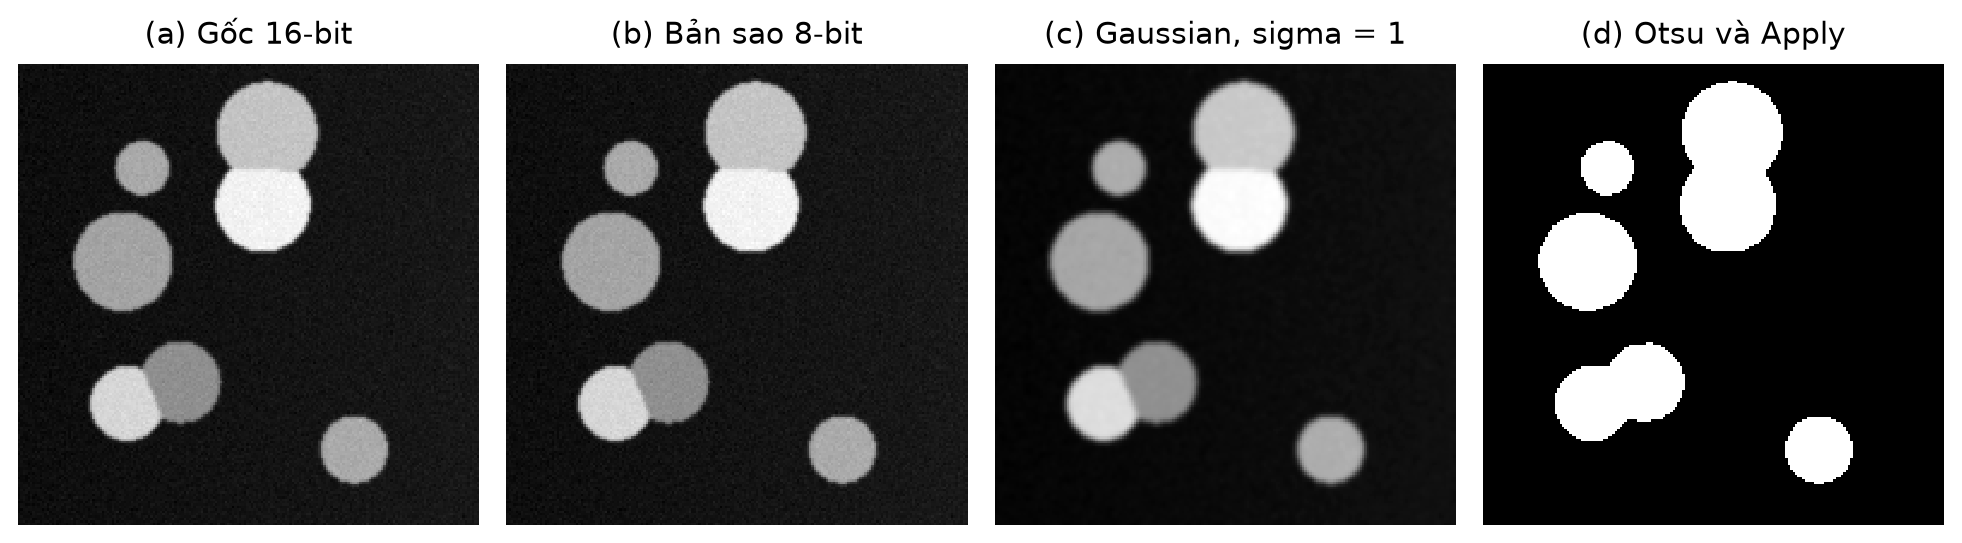
\includegraphics[width=\linewidth]{figures/manual_preprocess.png}
\caption{Ảnh thật của từng bước thực hành: nguồn 16-bit, bản sao 8-bit, Gaussian và nhị phân Otsu. Giống nhau về cách nhìn không có nghĩa dữ liệu không đổi.}\label{fig:manual-preprocess}
\end{figure}

\section{Bước 4: khảo sát co, giãn, mở, đóng và tái tạo}
Từ \emph{các bản sao độc lập của binary}, mở \textbf{MorphoLibJ $\to$ Filtering $\to$ Morphological Filters}. Operation chọn phép toán; Element chọn hình SE; Radius chọn tầm lân cận. Square r=4 có cạnh $2r+1=9$, không phải 4 pixel. Mỗi cửa sổ tính \emph{một} pixel đầu ra: co lấy MIN, giãn lấy MAX trên các vị trí được SE chọn; không giảm kích thước ảnh.

Opening co rồi giãn, loại chi tiết trắng nhỏ; Closing giãn rồi co, khép khe hoặc lỗ tối nhỏ. Mở không tạo thêm tiền cảnh ngoài ảnh gốc; đóng có thể nối vật gần nhau. Radius lớn dễ nhìn tác dụng nhưng cũng dễ làm mất vật thật. Các ảnh học thử trong Hình~\ref{fig:manual-morphology} ghi rõ bán kính khác nhau.
\begin{figure}[htbp]\centering
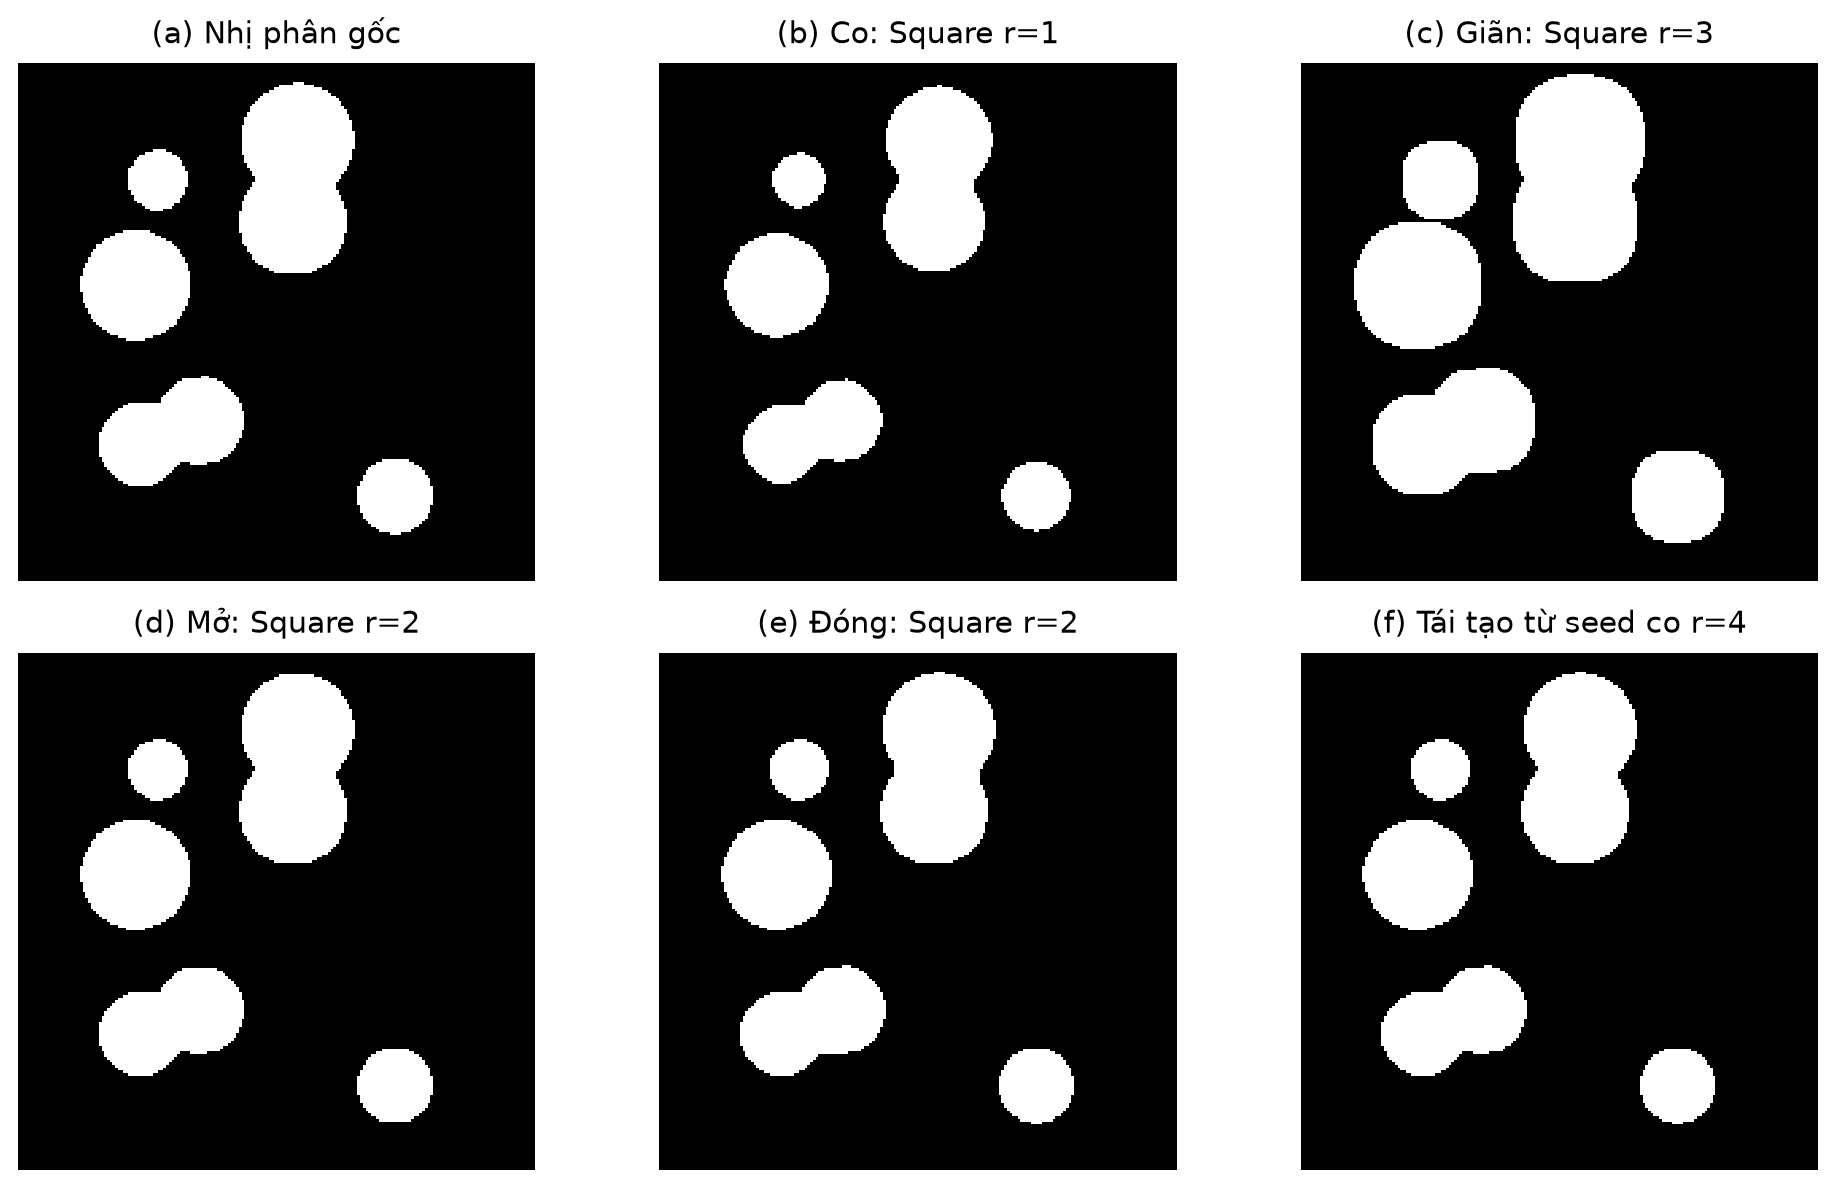
\includegraphics[width=\linewidth]{figures/manual_morphology.png}
\caption{Các kết quả Fiji do người học thực hiện. Đây là khảo sát thao tác với bán kính ghi trên từng ô; bộ so sánh cùng bán kính nằm ở Hình~\ref{fig:morphology}.}\label{fig:manual-morphology}
\end{figure}

Để mở bằng tái tạo, co binary thành seed, rồi gọi \textbf{Filtering $\to$ Morphological Reconstruction}: Marker Image=seed đã co, Mask Image=binary gốc, Type=By Dilation, Connectivity=4. Phép giãn bị mask chặn và lặp tới ổn định. Vùng liên thông còn ít nhất một seed được khôi phục; vùng mất seed hoàn toàn bị loại. Marker của tái tạo là ảnh khởi tạo cường độ, khác ảnh ID marker cho Watershed ở bước sau.

\section{Bước 5--6: làm sạch mask và đếm vùng liên thông}
Trên kết quả tái tạo, \textbf{Filtering $\to$ Fill Holes (Binary/Gray)} lấp nền kín bên trong vật. Nó không lấp khoảng trống thông ra nền ngoài. Sau đó \textbf{Binary Images $\to$ Size Opening 2D/3D}, Min Pixel Number=25, loại vùng liên thông nhỏ hơn 25 pixel, giữ nguyên hình dạng vùng còn lại. Hai vật dính nhau được tính chung diện tích. Lưu kết quả thành mask; nếu ảnh sạch, các bước này có thể không thay đổi pixel.

Chọn mask, \textbf{Binary Images $\to$ Connected Components Labeling}: Connectivity=4, Type=float. Đầu ra có năm ID vì mỗi cặp đang chạm nhau vẫn là một vùng. Chọn ảnh nhãn, \textbf{Analyze $\to$ Analyze Regions}, tích Area, Bounding Box, Centroid. Các ô tích chỉ yêu cầu tính cột, không lọc hoặc xóa vật. Area là diện tích, Centroid là trung bình tọa độ pixel, Bounding Box là hộp bao; gốc tọa độ ở góc trên trái, x tăng sang phải, y tăng xuống dưới.
\begin{figure}[htbp]\centering
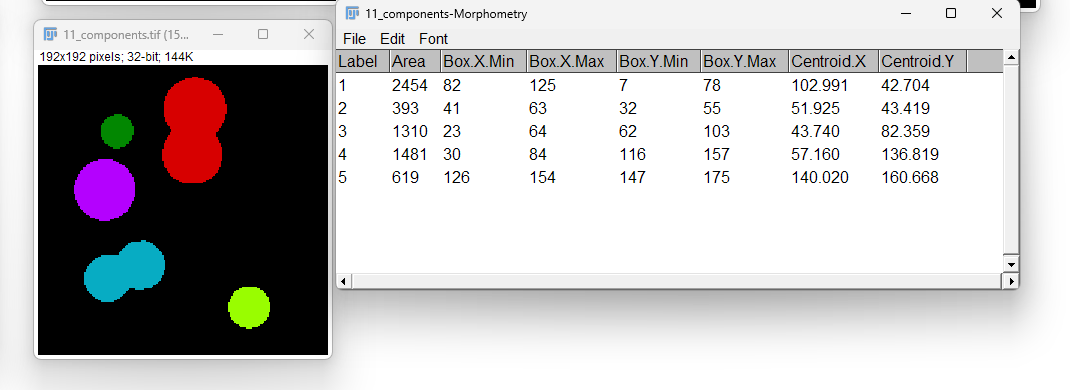
\includegraphics[width=0.94\linewidth]{figures/ui_components.png}
\caption{Ảnh chụp Fiji trong lần thực hành: năm vùng liên thông và bảng đo. Vùng đỏ gộp hai vật phía trên; vùng xanh ngọc gộp hai vật phía dưới.}\label{fig:manual-components}
\end{figure}

\section{Bước 7--8: distance, cực đại và marker có ID}
\begin{enumerate}[leftmargin=*,itemsep=3pt]
\item Chọn lại \emph{mask nhị phân 8-bit 0/255}, không chọn components. \textbf{Process $\to$ Binary $\to$ Options}: EDM output=32-bit; chạy \textbf{Distance Map}. Mỗi pixel trong vật nhận khoảng cách Euclid tới nền gần nhất. Đầu ra cần float để giữ khoảng cách lẻ; không chuyển distance 8-bit sang float sau khi đã mất độ chính xác.
\item Chọn distance 32-bit; \textbf{MorphoLibJ $\to$ Minima and Maxima $\to$ Extended Min \& Max}: \textbf{Extended Maxima}, Dynamic=2, Connectivity=4. h lọc độ nổi của cực đại, không phải số đối tượng hay ngưỡng cường độ tuyệt đối. Minima sẽ tìm vùng thấp, gồm nền, nên không dùng cho bước này.
\item Chọn \emph{ảnh kết quả mới của plugin}, là mask cực đại 8-bit. Không gán nhãn lên bản sao distance còn 32-bit. Kiểm tra ngoài cực đại=0, cực đại=255; Inverting LUT có thể làm màu nhìn ngược giá trị.
\item Chạy Connected Components Labeling trên mask cực đại: Connectivity=4, Type=float. Kết quả có bảy ID marker; một marker có thể gồm nhiều pixel. Không chỉnh marker theo ground truth để ép số lượng mong muốn.
\end{enumerate}
\begin{figure}[htbp]\centering
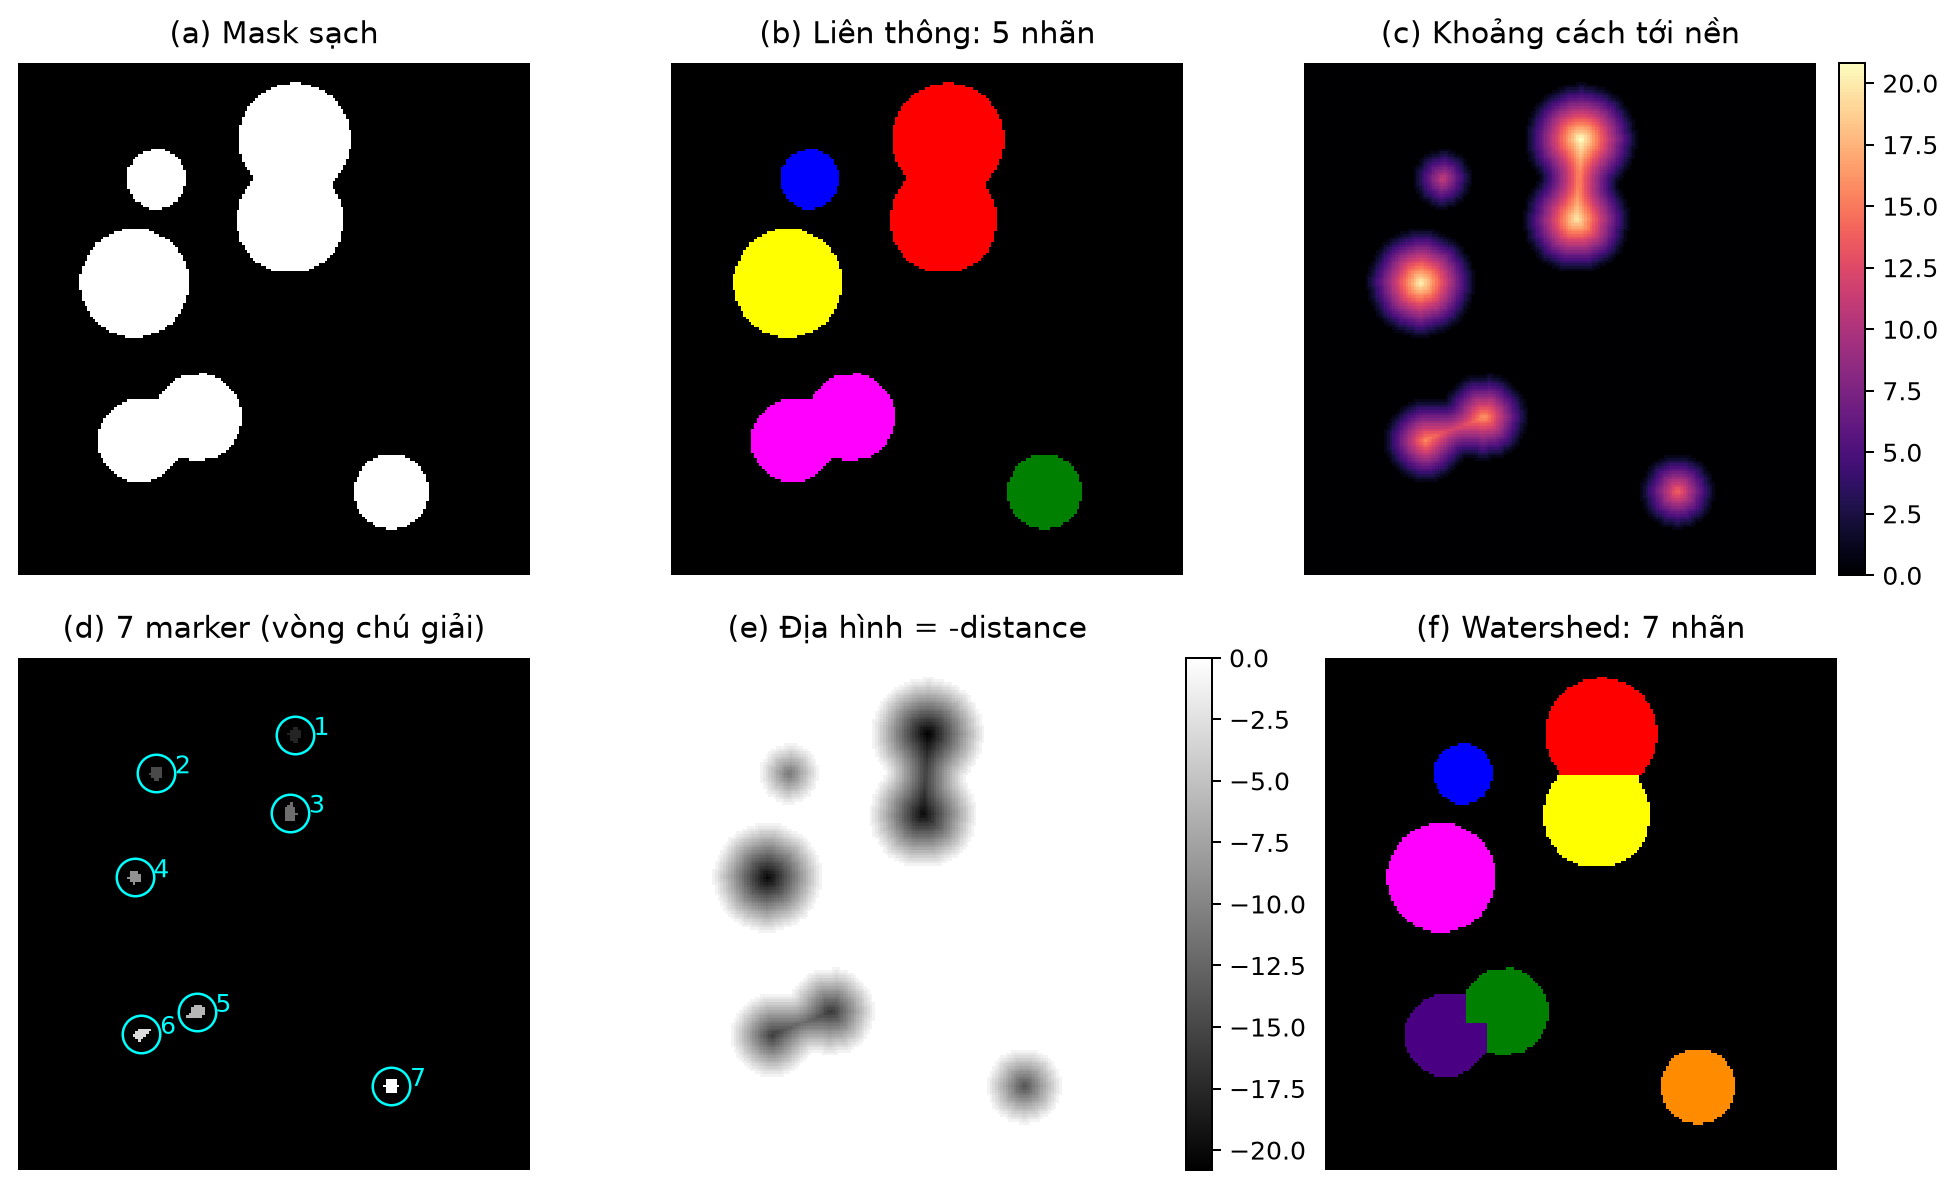
\includegraphics[width=\linewidth]{figures/manual_watershed.png}
\caption{Chuỗi dữ liệu thực hành: mask, năm thành phần, distance float, bảy marker, địa hình âm và nhãn Watershed. Vòng xanh ở ô marker chỉ chú giải vị trí, không thay kích thước seed trong TIFF.}\label{fig:manual-watershed}
\end{figure}

\section{Bước 9: địa hình âm và Marker-controlled Watershed}
Nhân bản distance, \textbf{Process $\to$ Math $\to$ Multiply}, nhập $-1$, nhận $E=-D$. Nền bằng 0, trong vật âm; tâm sâu hơn là vùng thấp. Chỉnh Brightness/Contrast chỉ để nhìn; Invert LUT không thay thế phép nhân.

Trong nhóm \textbf{MorphoLibJ $\to$ Segmentation}, mở lệnh \textbf{Marker-controlled Watershed}. Chọn Input là elevation, Marker là ảnh bảy ID và Mask là mặt nạ sạch. Đặt Compactness=0; bỏ Binary markers, Calculate dams và Use diagonal connectivity. Nhãn marker giữ ID riêng, không tạo đường nền phân cách, liên thông 4. Kết quả có bảy nhãn, được đo lại bằng Analyze Regions. Nhãn khác màu không có nghĩa khác vật; Spectrum từng làm nền và một nhãn trùng màu, nhưng bảng vẫn đủ bảy ID. LUT chỉ đổi cách hiển thị.

Kiểm tra tệp lưu phát hiện \path{15_elevation.tif} còn là bản distance dương trước phép nhân. Nhóm giữ nguyên bản này để truy vết và xuất lại $E=-D$ trong bộ minh chứng. Chạy lại MorphoLibJ trên $-D$ với marker/mask đã lưu cho nhãn trùng kết quả làm tay sau ghép ID, không pixel bất đồng; dùng $+D$ lệch 1915 pixel. Vì vậy báo cáo dùng địa hình âm đã kiểm chứng, không chỉ dựa vào tên tệp. Nhãn dự đoán làm tay không bị thay thế.

\section{Bước 10: đo IoU/Dice ngay trong Fiji}
Mở nhãn đúng; Duplicate cả nhãn đúng và nhãn dự đoán. Trên hai bản sao, tắt \textbf{Scale When Converting}, chuyển 8-bit để giữ nguyên ID nhỏ 0--7; Threshold $\to$ Set chọn 1--7, Apply thành vật 255/nền 0. Không dùng Otsu trên ID nhãn. Giữ nguyên hai TIFF nhãn gốc để đánh giá từng đối tượng bằng Python.

Trong nhóm \textbf{Analyze}, chọn \textbf{Label Overlap Measures}. Source là GT foreground, Target là Prediction foreground; bật Jaccard index và Dice coefficient. Vì mask chỉ còn nhãn tiền cảnh 255, bảng all-labels và individual-labels cho cùng số. Label 255 không phải 255 vật. Phép đo này đánh giá vật/nền, không tự chấm lỗi tách từng vật đang dính.
\begin{figure}[htbp]\centering
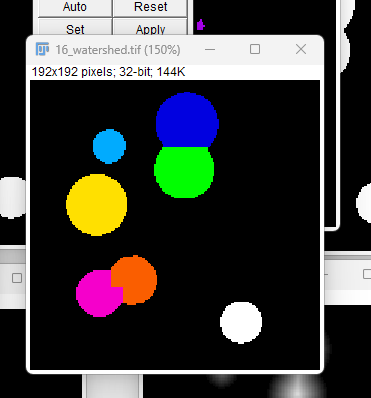
\includegraphics[width=0.28\linewidth]{figures/ui_watershed.png}\hfill
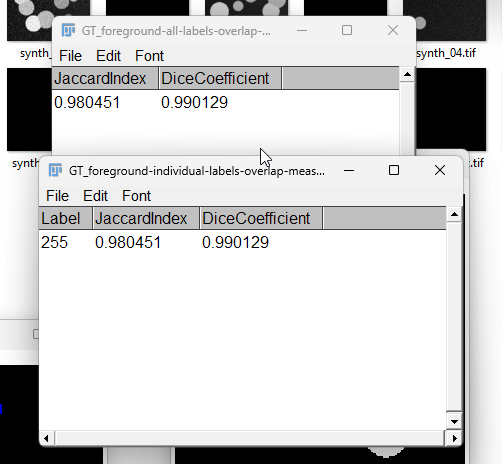
\includegraphics[width=0.66\linewidth]{figures/ui_overlap.png}
\caption{Ảnh chụp kết quả làm tay: nhãn Watershed hiển thị màu và bảng overlap Fiji, Jaccard=0,980451; Dice=0,990129. Các màu chỉ là LUT.}\label{fig:manual-ui-result}
\end{figure}

\begin{figure}[htbp]\centering
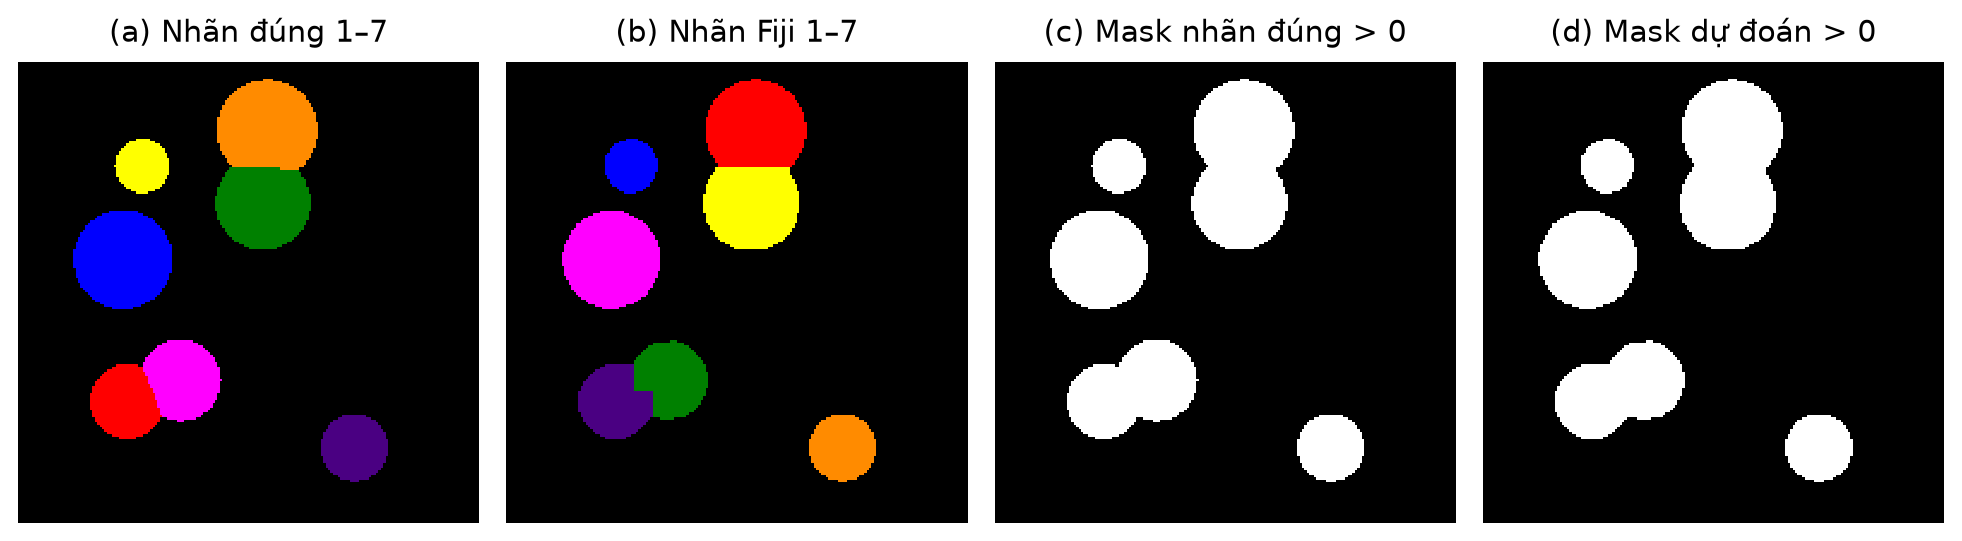
\includegraphics[width=\linewidth]{figures/manual_evaluation.png}
\caption{Nhãn đúng, nhãn Fiji và hai mask tiền cảnh được dùng đo. Nhị phân hóa làm mất ID từng vật nên chỉ dùng hai mask cuối để chấm tiền cảnh.}\label{fig:manual-evaluation}
\end{figure}

\begin{table}[htbp]\centering\small
\caption{Chấm kết quả Fiji làm tay: GUI và code độc lập khớp trong sai số hiển thị.}\label{tab:manual-metrics}
\begin{tabularx}{\linewidth}{X r r}\toprule
Chỉ số & Fiji GUI & Python chấm TIFF Fiji\\\midrule
IoU/Jaccard tiền cảnh & 0,980451 & 0,98045089\\
Dice tiền cảnh & 0,990129 & 0,99012896\\
Số nhãn dự đoán & 7 & 7\\
F1 đối tượng tại IoU $\geq 0,5$ & Không đo ở bảng này & 1,000000\\
TP / FP / FN & Không đo ở bảng này & 7 / 0 / 0\\\bottomrule
\end{tabularx}\end{table}
F1=1 chỉ có nghĩa đủ bảy cặp ghép hợp lệ, không phải mọi pixel đúng. Biên còn khác nhãn đúng nên IoU thấp hơn 1. Kết quả thao tác tay được tách khỏi baseline native tự động (IoU khoảng 0,980132) và Python mặc định (khoảng 0,981397). Một ảnh đơn giản minh họa quy trình; đánh giá nhiều ảnh nằm ở Chương~\ref{chap:experiments}.

\section{Tự động hóa sau khi hiểu thao tác}
Groovy là ngôn ngữ chạy trên Java, có thể gọi API ImageJ/MorphoLibJ trong Fiji Script Editor. \textbf{File $\to$ New $\to$ Script}, mở \path{fiji/Full_Pipeline_Tutorial.groovy}, chọn Language=Groovy rồi Run để chạy từ ảnh gốc theo giao thức cố định. \path{fiji/ReplayWatershed.groovy} chỉ chạy lại bước Watershed từ ba TIFF. Recorder tại \textbf{Plugins $\to$ Macros $\to$ Record} giúp ghi các lệnh menu có hỗ trợ. Chạy lại trên bản sao để kiểm tra script, không giả định Recorder ghi được mọi thao tác.

Trong đánh giá tự động, Fiji shared nhận cùng elevation/markers/mask với Python để kiểm chứng bước Watershed. Fiji native tự xử lý từ ảnh xám chuẩn hóa, dùng 8-bit, SE vuông và ImageJ EDM. Python mặc định dùng float, SE đĩa và EDT tự cài. Khác biệt cả pipeline không được quy về riêng hàm Watershed. Thời gian native có ghi TIFF, không so trực tiếp với thời gian kernel shared để công bố tốc độ.
